\documentclass{sciposter}
\usepackage{lipsum}
\usepackage{epsfig}
\usepackage{amsmath}
\usepackage{amssymb}
\usepackage{multicol}
\usepackage{graphicx,url}
\usepackage[portuges, brazil]{babel}   
\usepackage[utf8]{inputenc}
%\usepackage{fancybullets}
\newtheorem{Def}{Definition}


\title{Classic Methods on \\Color Based Ball Tracking}
%Título do projeto

\author{Breno Leite\\Guilherme Leite}
%nome dos autores

\institute 
{Introduction to Computer Vision\\
Instituto de Computa\c{c}\~ao -- UNICAMP}
%Nome e endereço da Instituição

\email{{brenolleite, guilherme.vieira.leite},{(@gmail.com})}
% Onde você coloca os emails dos integrantes


%\date is unused by the current \maketitle

\rightlogo[1]{ic-logo}
\leftlogo[1]{unicamp-logo}
% Exibe os logos (direita e esquerda) 
% Procure usar arquivos png ou jpg, e de preferencia mantenha na mesma pasta do .tex
%%%%%%%%%%%%%%%%%%%%%%%%%%%%%%%%%%%%%%%%%%%%%%%%%%%%%%%%%%%%%%%%%%%%%%%%%%%%%%%%
%%% Begin of Document



\begin{document}
%define conference poster is presented at (appears as footer)

%\LEFTSIDEfootlogo  
% Uncomment to put footer logo on left side, and 
% conference name on right side of footer

% Some examples of caption control (remove % to check result)

%\renewcommand{\algorithmname}{Algoritme} % for Dutch

%\renewcommand{\mastercapstartstyle}[1]{\textit{\textbf{#1}}}
%\renewcommand{\algcapstartstyle}[1]{\textsc{\textbf{#1}}}
%\renewcommand{\algcapbodystyle}{\bfseries}
%\renewcommand{\thealgorithm}{\Roman{algorithm}}

\maketitle

%%% Begin of Multicols-Enviroment
\begin{multicols}{3}

%%% Abstract

%%% Introduction
\section{Motivation}

Ball tracking is a classical problem both for its simplicity and applications. Nowadays it is used in sports events to automatically track the focus of the action and game score, its also widely used in robotics, specially in robocup's soccer competitions.

\section{Methodology}

Our experiments derived from the following setup:

\begin{itemize}

\item Fixed camera;
\item Two yellow balls;
\item One blue ball;

\end{itemize}

\bigbreak
We also covered the following scenarios:

\begin{itemize}

\item Single colored ball;
\item Two different colored balls;
\item Two same color balls;
\item All three balls;
\item Other objects with the balls;
\item Collision between same color balls;
\item Real world application;

\end{itemize}

\section{Experiments}

We approached all the scenarios listed above in a incremental manner in complexity order. Below are listed 

\bigbreak
A single colored ball:

\begin{figure}[!h]
	\centering
			\setlength{\fboxsep}{1pt}
			\setlength{\fboxrule}{1pt}
			\fbox{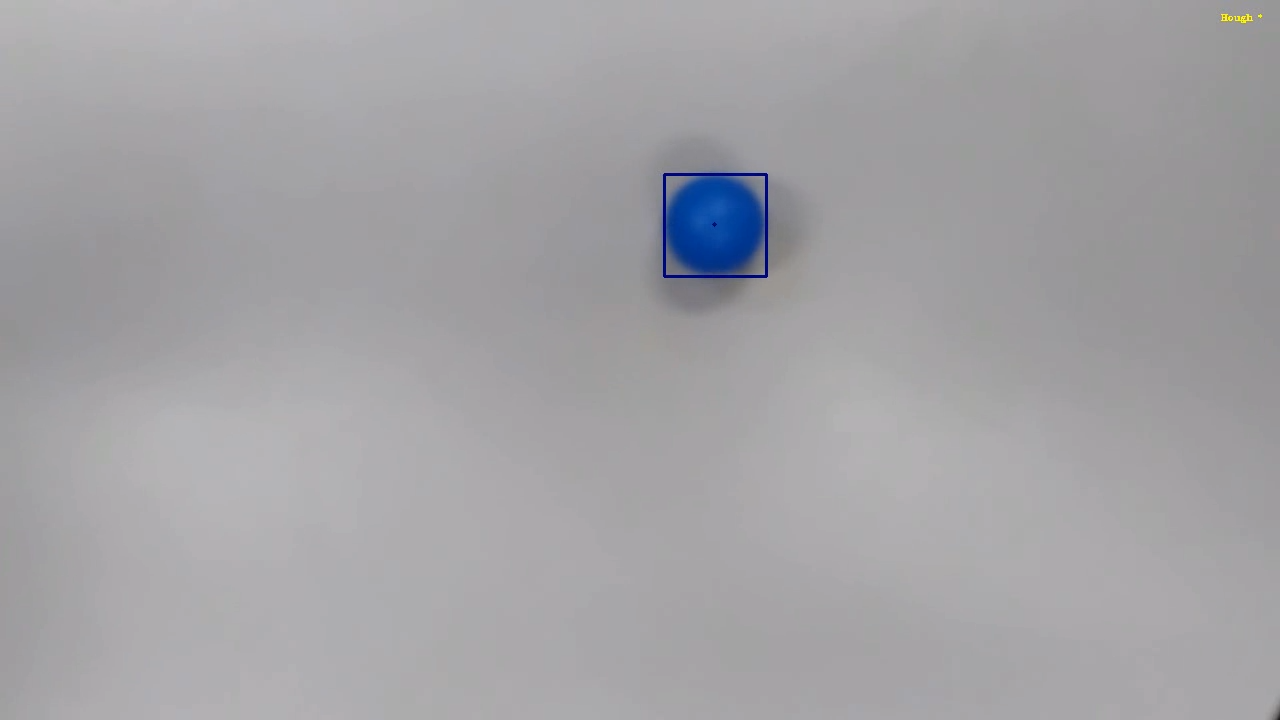
\includegraphics[scale=0.5]{images/single_color}}
	\caption{Track of a single colored ball}
	\label{fig:single_color}
\end{figure}

Two different colored balls:

\begin{figure}[!h]
	\centering
			\setlength{\fboxsep}{1pt}
			\setlength{\fboxrule}{1pt}
			\fbox{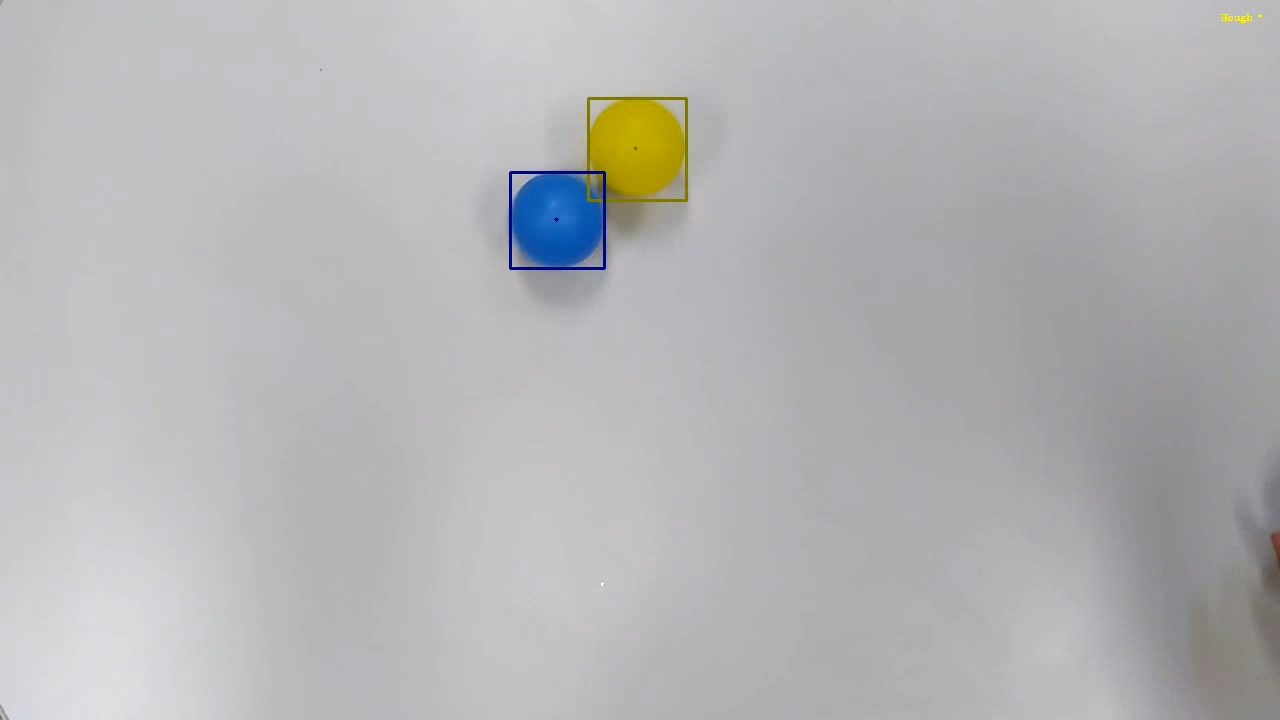
\includegraphics[scale=0.5]{images/diff_color}}
	\caption{Track of two differently colored balls}
	\label{fig:diff_color}
\end{figure}

Two different colored balls:

\begin{figure}[!h]
	\centering
			\setlength{\fboxsep}{1pt}
			\setlength{\fboxrule}{1pt}
			\fbox{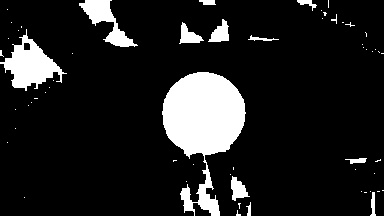
\includegraphics[scale=0.5]{images/two_same}}
	\caption{Track of two same color balls}
	\label{fig:two_same}
\end{figure}

All three colored balls:

\begin{figure}[!h]
	\centering
			\setlength{\fboxsep}{1pt}
			\setlength{\fboxrule}{1pt}
			\fbox{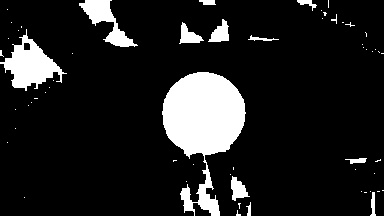
\includegraphics[scale=0.5]{images/three_balls}}
	\caption{Track of all three colored balls}
	\label{fig:three_balls}
\end{figure}

Mixed shaped objects with the balls:

\begin{figure}[!h]
	\centering
			\setlength{\fboxsep}{1pt}
			\setlength{\fboxrule}{1pt}
			\fbox{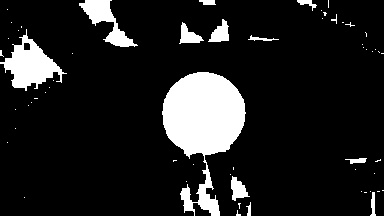
\includegraphics[scale=0.5]{images/mixed_shape}}
	\caption{Track of the balls alongside mixed shaped objects}
	\label{fig:mixed_shape}
\end{figure}

Collision between same color balls:

\begin{figure}[!h]
	\centering
			\setlength{\fboxsep}{1pt}
			\setlength{\fboxrule}{1pt}
			\fbox{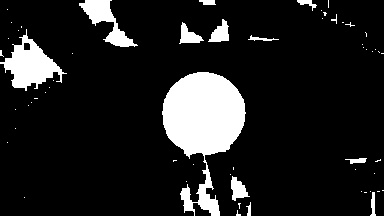
\includegraphics[scale=0.5]{images/coll_same_color}}
	\caption{Track of two same color balls with collision}
	\label{fig:call_same_color}
\end{figure}

Real world application:

\begin{figure}[!h]
	\centering
			\setlength{\fboxsep}{1pt}
			\setlength{\fboxrule}{1pt}
			\fbox{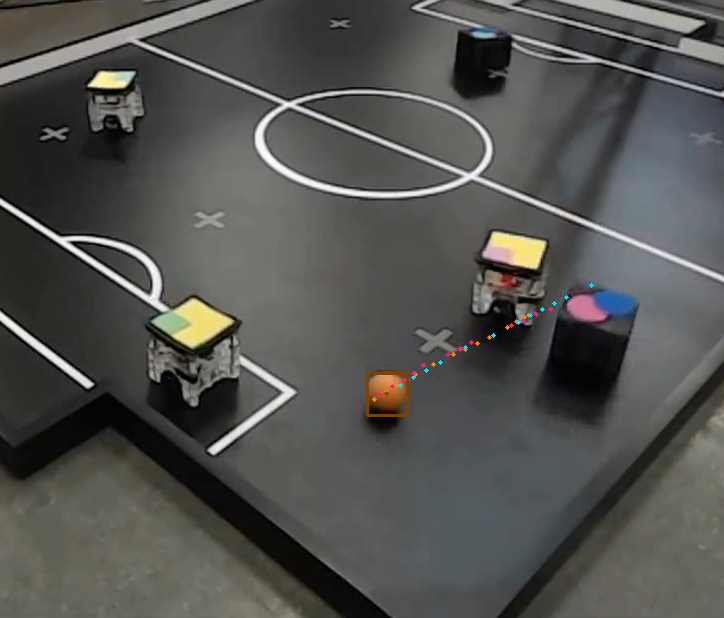
\includegraphics[scale=0.5]{images/robocup_1}}
	\caption{Track of one colored ball in the Robocup soccer competition}
	\label{fig:robocup_1}
\end{figure}

\section{Conclusions}

As seem previously the classic methods can present good results in a controlled environment, but lack the robustness to perform flawlessly in a noisy scenario. To perform in a such complex scenarios a different set of tools are used in the literature, from physics model to deep neural networks.

%%% References

%% Note: use of BibTeX als works!!

\bibliographystyle{plain}
\begin{thebibliography}{1}

\bibitem{Flusser:Suk:93}
J.~Flusser and T.~Suk.
\newblock Pattern recognition by affine moment invariants.
\newblock {\em Pattern Recognition}, 26:167--174, 1993.

\bibitem{Hu:62}
M.~K. Hu.
\newblock Visual pattern recognition by moment invariants.
\newblock {\em IRE Transactions on Information Theory}, IT-8:179--187, 1962.

\bibitem{maragos89:_patter}
P.~Maragos.
\newblock Pattern spectrum and multiscale shape representation.
\newblock {\em IEEE Trans. Patt. Anal. Mach. Intell.}, 11:701--715, 1989.

\bibitem{Meijster:Wilkinson:PAMI}
A.~Meijster and M.~H.~F. Wilkinson.
\newblock A comparison of algorithms for connected set openings and closings.
\newblock {\em IEEE Trans. Patt. Anal. Mach. Intell.}, 24(4):484--494, 2002.

\bibitem{Nacken:thesis}
P.~F.~M. Nacken.
\newblock {\em Image Analysis Methods Based on Hierarchies of Graphs and
  Multi-Scale Mathematical Morphology}.
\newblock PhD thesis, University of Amsterdam, Amsterdam, The Netherlands,
  1994.

\end{thebibliography}

\end{multicols}

\end{document}